% Options for packages loaded elsewhere
\PassOptionsToPackage{unicode}{hyperref}
\PassOptionsToPackage{hyphens}{url}
%
\documentclass[
]{article}
\usepackage{amsmath,amssymb}
\usepackage{lmodern}
\usepackage{ifxetex,ifluatex}
\ifnum 0\ifxetex 1\fi\ifluatex 1\fi=0 % if pdftex
  \usepackage[T1]{fontenc}
  \usepackage[utf8]{inputenc}
  \usepackage{textcomp} % provide euro and other symbols
\else % if luatex or xetex
  \usepackage{unicode-math}
  \defaultfontfeatures{Scale=MatchLowercase}
  \defaultfontfeatures[\rmfamily]{Ligatures=TeX,Scale=1}
\fi
% Use upquote if available, for straight quotes in verbatim environments
\IfFileExists{upquote.sty}{\usepackage{upquote}}{}
\IfFileExists{microtype.sty}{% use microtype if available
  \usepackage[]{microtype}
  \UseMicrotypeSet[protrusion]{basicmath} % disable protrusion for tt fonts
}{}
\makeatletter
\@ifundefined{KOMAClassName}{% if non-KOMA class
  \IfFileExists{parskip.sty}{%
    \usepackage{parskip}
  }{% else
    \setlength{\parindent}{0pt}
    \setlength{\parskip}{6pt plus 2pt minus 1pt}}
}{% if KOMA class
  \KOMAoptions{parskip=half}}
\makeatother
\usepackage{xcolor}
\IfFileExists{xurl.sty}{\usepackage{xurl}}{} % add URL line breaks if available
\IfFileExists{bookmark.sty}{\usepackage{bookmark}}{\usepackage{hyperref}}
\hypersetup{
  pdftitle={Notes on: Combining evidence from different GWAS studies for binary traits},
  pdfauthor={Ziang Zhang, Lei Sun},
  hidelinks,
  pdfcreator={LaTeX via pandoc}}
\urlstyle{same} % disable monospaced font for URLs
\usepackage[margin=1in]{geometry}
\usepackage{color}
\usepackage{fancyvrb}
\newcommand{\VerbBar}{|}
\newcommand{\VERB}{\Verb[commandchars=\\\{\}]}
\DefineVerbatimEnvironment{Highlighting}{Verbatim}{commandchars=\\\{\}}
% Add ',fontsize=\small' for more characters per line
\usepackage{framed}
\definecolor{shadecolor}{RGB}{248,248,248}
\newenvironment{Shaded}{\begin{snugshade}}{\end{snugshade}}
\newcommand{\AlertTok}[1]{\textcolor[rgb]{0.94,0.16,0.16}{#1}}
\newcommand{\AnnotationTok}[1]{\textcolor[rgb]{0.56,0.35,0.01}{\textbf{\textit{#1}}}}
\newcommand{\AttributeTok}[1]{\textcolor[rgb]{0.77,0.63,0.00}{#1}}
\newcommand{\BaseNTok}[1]{\textcolor[rgb]{0.00,0.00,0.81}{#1}}
\newcommand{\BuiltInTok}[1]{#1}
\newcommand{\CharTok}[1]{\textcolor[rgb]{0.31,0.60,0.02}{#1}}
\newcommand{\CommentTok}[1]{\textcolor[rgb]{0.56,0.35,0.01}{\textit{#1}}}
\newcommand{\CommentVarTok}[1]{\textcolor[rgb]{0.56,0.35,0.01}{\textbf{\textit{#1}}}}
\newcommand{\ConstantTok}[1]{\textcolor[rgb]{0.00,0.00,0.00}{#1}}
\newcommand{\ControlFlowTok}[1]{\textcolor[rgb]{0.13,0.29,0.53}{\textbf{#1}}}
\newcommand{\DataTypeTok}[1]{\textcolor[rgb]{0.13,0.29,0.53}{#1}}
\newcommand{\DecValTok}[1]{\textcolor[rgb]{0.00,0.00,0.81}{#1}}
\newcommand{\DocumentationTok}[1]{\textcolor[rgb]{0.56,0.35,0.01}{\textbf{\textit{#1}}}}
\newcommand{\ErrorTok}[1]{\textcolor[rgb]{0.64,0.00,0.00}{\textbf{#1}}}
\newcommand{\ExtensionTok}[1]{#1}
\newcommand{\FloatTok}[1]{\textcolor[rgb]{0.00,0.00,0.81}{#1}}
\newcommand{\FunctionTok}[1]{\textcolor[rgb]{0.00,0.00,0.00}{#1}}
\newcommand{\ImportTok}[1]{#1}
\newcommand{\InformationTok}[1]{\textcolor[rgb]{0.56,0.35,0.01}{\textbf{\textit{#1}}}}
\newcommand{\KeywordTok}[1]{\textcolor[rgb]{0.13,0.29,0.53}{\textbf{#1}}}
\newcommand{\NormalTok}[1]{#1}
\newcommand{\OperatorTok}[1]{\textcolor[rgb]{0.81,0.36,0.00}{\textbf{#1}}}
\newcommand{\OtherTok}[1]{\textcolor[rgb]{0.56,0.35,0.01}{#1}}
\newcommand{\PreprocessorTok}[1]{\textcolor[rgb]{0.56,0.35,0.01}{\textit{#1}}}
\newcommand{\RegionMarkerTok}[1]{#1}
\newcommand{\SpecialCharTok}[1]{\textcolor[rgb]{0.00,0.00,0.00}{#1}}
\newcommand{\SpecialStringTok}[1]{\textcolor[rgb]{0.31,0.60,0.02}{#1}}
\newcommand{\StringTok}[1]{\textcolor[rgb]{0.31,0.60,0.02}{#1}}
\newcommand{\VariableTok}[1]{\textcolor[rgb]{0.00,0.00,0.00}{#1}}
\newcommand{\VerbatimStringTok}[1]{\textcolor[rgb]{0.31,0.60,0.02}{#1}}
\newcommand{\WarningTok}[1]{\textcolor[rgb]{0.56,0.35,0.01}{\textbf{\textit{#1}}}}
\usepackage{graphicx}
\makeatletter
\def\maxwidth{\ifdim\Gin@nat@width>\linewidth\linewidth\else\Gin@nat@width\fi}
\def\maxheight{\ifdim\Gin@nat@height>\textheight\textheight\else\Gin@nat@height\fi}
\makeatother
% Scale images if necessary, so that they will not overflow the page
% margins by default, and it is still possible to overwrite the defaults
% using explicit options in \includegraphics[width, height, ...]{}
\setkeys{Gin}{width=\maxwidth,height=\maxheight,keepaspectratio}
% Set default figure placement to htbp
\makeatletter
\def\fps@figure{htbp}
\makeatother
\setlength{\emergencystretch}{3em} % prevent overfull lines
\providecommand{\tightlist}{%
  \setlength{\itemsep}{0pt}\setlength{\parskip}{0pt}}
\setcounter{secnumdepth}{5}
\usepackage{amsmath,amsthm, amssymb}
\usepackage{booktabs}
\usepackage{longtable}
\usepackage{array}
\usepackage{multirow}
\usepackage{wrapfig}
\usepackage{float}
\usepackage{colortbl}
\usepackage{pdflscape}
\usepackage{tabu}
\usepackage{threeparttable}
\usepackage{threeparttablex}
\usepackage[normalem]{ulem}
\usepackage{makecell}
\usepackage{xcolor}
\ifluatex
  \usepackage{selnolig}  % disable illegal ligatures
\fi
\newlength{\cslhangindent}
\setlength{\cslhangindent}{1.5em}
\newlength{\csllabelwidth}
\setlength{\csllabelwidth}{3em}
\newenvironment{CSLReferences}[2] % #1 hanging-ident, #2 entry spacing
 {% don't indent paragraphs
  \setlength{\parindent}{0pt}
  % turn on hanging indent if param 1 is 1
  \ifodd #1 \everypar{\setlength{\hangindent}{\cslhangindent}}\ignorespaces\fi
  % set entry spacing
  \ifnum #2 > 0
  \setlength{\parskip}{#2\baselineskip}
  \fi
 }%
 {}
\usepackage{calc}
\newcommand{\CSLBlock}[1]{#1\hfill\break}
\newcommand{\CSLLeftMargin}[1]{\parbox[t]{\csllabelwidth}{#1}}
\newcommand{\CSLRightInline}[1]{\parbox[t]{\linewidth - \csllabelwidth}{#1}\break}
\newcommand{\CSLIndent}[1]{\hspace{\cslhangindent}#1}

\title{\textbf{Notes on: Combining evidence from different GWAS studies
for binary traits}}
\author{Ziang Zhang, Lei Sun}
\date{}

\begin{document}
\maketitle

\newcommand{\p}{\text{P}}
\newcommand{\E}{\mathbb{E}}
\newcommand{\Var}{\text{Var}}

\hypertarget{introduction}{%
\section{Introduction:}\label{introduction}}

For most human traits, genetic effects from specific SNP only have small
effect sizes (Evangelou and Ioannidis 2013). Therefore, practitioners
often aggregate the GWAS results from different studies through
meta-analysis or mega-analysis in order to achieve higher power.
Aggregation through p-values is a commonly used example of meta-analysis
method. For example when there are several different datasets,
practitioners sometimes will first carry out a comprehensive study using
one dataset, and only follow up with the SNPs that have the highest
significance levels (Begum et al. 2012). Another example would be
multi-trait analysis which contains a joint analysis of multiple related
traits, in order to boost the statistical power (Turley et al. 2018). In
this note, we would like to consider some problems that practitioners
may encounter when applying such procedures on the analysis of binary
traits.

With examples of Wald test, we presented the phenomenon that the same
hypothesis test on different binary traits can have very different
distributions of p-value under the alternative hypothesis, hence very
different powers, even if the two traits have the same true SNP effect
and are analyzed using the same dataset.

In the next section, we will give a brief overview of Wald test for
Generalized Linear Models, with a short explanation of the rationale
behind the phenomenon we mentioned above. Then, we will follow with two
simulation studies to illustrate how this phenomenon is affecting the
analysis of binary trait, but not the analysis of continuous trait.

\hypertarget{wald-test-for-generalized-linear-models}{%
\section{Wald test for Generalized Linear
Models:}\label{wald-test-for-generalized-linear-models}}

Assume the generalized linear model (glm) has the following form:
\[\mathbb{E}(Y|X) = \mu = g^{-1}(\beta_0 + \beta_1 X_1 + \beta_2X_2) = g^{-1}(\eta),\]
where \(g(.)\) is a specific link function connecting the linear
predictor \(\eta\) with the mean function of \(Y\). In this case, the
fisher information matrix at \(\beta\) can be written as
\[I_n(\beta) = X^TW(\beta) X,\] where X denotes the design matrix and
\(W(\beta)\) is a diagonal matrix with each diagonal term depending on
the value of \(\beta\) unless \(g\) is identity function. Specifically,
the \(i^{th}\) diagonal term of W can be computed as
\[w_i=(\frac{\partial u_i}{\partial\eta_i})^2/\text{Var}(Y_i|X).\]

If the question of interest is to test the hypothesis \(H_0: \beta_2=0\)
using Wald test, the test statistic can be written as
\[T = \frac{(\hat{\beta_2})^2}{I_n^{-1}(\hat{\beta})_{[3,3]}},\] where
\(I_n^{-1}(\hat{\beta})_{[3,3]}\) denotes the third diagonal term of the
matrix \(I_n^{-1}(\hat{\beta})\) and \(\hat{\beta}\) is the MLE
estimator. Under the null hypothesis, \(T\) asymptotically follows a
Chi-Square distribution with 1 degree of freedom.

Under the alternative hypothesis that \(\beta_2 \neq 0\), the
non-centrality parameter of Wald test above can be computed as
\[\frac{\beta_2^2}{I_n^{-1}(\beta)_{[3,3]}},\] where \(\beta\) is the
vector of true values for the regression parameters \(\beta\). Since
\(I_n^{-1}(\beta)_{[3,3]}\) will not solely depend on \(\beta_2\) unless
\(g\) is identity. Therefore the power function of this Wald test will
not only depend on \(\beta_2\), but the whole vector \(\beta\).

Define \(d=-\frac{\beta_2}{\sqrt{I_n^{-1}(\beta)_{[3,3]}}}\), the
theoretical power of this Wald test at \(\beta\) can be computed as
\[1-\Phi(d+z_{a/2})+\Phi(d-z_{a/2}),\] where \(\Phi\) is the CDF of
standard normal and \(z_{a/2}\) is the \(a/2\) quantile of standard
normal.

In summary, this means that if we utilize Poisson regression to analyze
count traits (e.g.~number of cancers) or Logistic/Probit regression to
analyze binary traits (e.g.~disease status), powers of Wald test from
different studies can be dramatically different, even if the two studies
have the same effect size (i.e.~\(|\beta_2|\)) and the same set of
covariates \(\{X_{1i},X_{2i}\}_{i=1}^n\). The rationale behind this is
actually the classical contrast between
\textbf{statistical significance} measured by p-values and
\textbf{practical significance} measured by the size of the effect
\(|\beta_2|\). In Wald test, p-values are determined by both the
practical significance \(|\beta_2|\) and the standard error
\(\sqrt{I_n^{-1}(\beta)_{[3,3]}}\). Since the standard errors of the MLE
estimator will be different on the two studies, the conclusion drawn
from statistical significance may be inconsistent with the practical
significance of effects in the two studies.

\hypertarget{difference-between-continuous-trait-and-binary-trait}{%
\section{Difference between continuous trait and binary
trait:}\label{difference-between-continuous-trait-and-binary-trait}}

For the analysis of continuous trait, a natural option would be using
ordinary Gaussian linear regression model:
\[Y = \beta_0 + \beta_1 X_1 + \beta_2X_2+\epsilon,\] where
\(\epsilon \sim N(0,\sigma^2)\).

In this case, suppose the question of interest is testing \(\beta_2=0\),
the Wald test will have non-centrality parameter being
\[\frac{\beta_2^2}{\sigma^2[X^TX]^{-1}_{[33]}}.\]

Because the (inverse) information matrix \(\sigma^2[X^TX]^{-1}\) only
depends on the nuisance parameter \(\sigma\), power of this test will
not change as \(\beta_0\) or \(\beta_1\) change, as long as the nuisance
parameter is the same. This implies, if a SNP \(G\) has true effect
\(\beta_G\) being constant across two traits, then the power of testing
\(\beta_G = 0\) will be constant across two traits as well (assume same
\(\sigma^2\)). Therefore, the aggregation of evidences across traits
will be straightforward and smaller p value can be associated with
larger SNP effect.

On the other hand, if the target is to combine evidence across several
binary traits, the result will no longer be as straightforward. If
traits are generated from the following logistic regression model:
\[\text{P}(Y=1|X) = \beta_0 + \beta_1 X_1 + \beta_2X_2,\] In this case,
the corresponding non-centrality parameter of testing \(\beta_2=0\)
becomes \[\frac{\beta_2}{[X^TW_\beta X]^{-1}_{[33]}}.\]

Since \(g^{-1}(\eta)= \frac{\exp(\eta)}{1+\exp(\eta)}\) for logistic
regression, we can compute the i-th term of the diagonal matrix
\(W_\beta\) as
\[[W_\beta]_{ii} = f(\eta_i)=\frac{\exp(-\eta_i)}{(1+\exp(-\eta_i))^2}.\]
The function \(f(.)\) represents the density function of standard
logistic distribution, and the term \(\eta_i\) is the i-th linear
predictor. This implies the non-centrality parameter, hence the power
will depend on every parameter in the model, not just on the parameter
of interest \(\beta_2\).

An important consequence of this phenomenon is that, the magnitude of p
values (statistical significance) will not reflect the magnitude of the
SNP effects (pratical significance), even if the two studies are carried
out using one common dataset. For example, if a SNP has effect
\(\beta_G\) on both traits, it may show significance on only one trait
because of the difference in the covariate effect such as gender or
race.

\hypertarget{simulation-with-gaussian-linear-regression-model}{%
\section{Simulation with Gaussian linear regression
model:}\label{simulation-with-gaussian-linear-regression-model}}

Assume a dataset of size \(n=1000\) has been collected. The dataset
contains the information of a continuous covariate Z, a SNP G, and two
continuous traits (A and B). For simplicity, assume this SNP follows
hardy weinberg equilibrium (HWE) with minor allele frequency (MAF)
\(0.3\), and the covariate \(Z\) has been centered such that
\(Z\sim N(0,\sigma=3)\).

Furthermore, we assume that the generating models for each trait are the
followings: \[\textbf{A}:Y = -0.5 + 0.8Z + 0.3G + \epsilon,\]
\[\textbf{B}: Y = -0.5 + 0.1Z + 0.3G + \epsilon,\] where the noise term
\(\epsilon\) follows \(N(0,3)\) in both models.

To test the null hypothesis \(H_0: \beta_G = 0\), a Wald test can be
carried out for each trait (with \(\alpha=0.05\) for simplicity). Using
the formula from above, we can compute the theoretical power of each
trait:

\begin{Shaded}
\begin{Highlighting}[]
\DocumentationTok{\#\#\# Simulated the common Z and G}
\FunctionTok{set.seed}\NormalTok{(}\DecValTok{100}\NormalTok{,}\AttributeTok{sample.kind =} \StringTok{"Rounding"}\NormalTok{)}
\NormalTok{N }\OtherTok{\textless{}{-}} \DecValTok{1000}
\NormalTok{G }\OtherTok{\textless{}{-}} \FunctionTok{sample}\NormalTok{(}\FunctionTok{c}\NormalTok{(}\DecValTok{0}\NormalTok{,}\DecValTok{1}\NormalTok{,}\DecValTok{2}\NormalTok{),}\AttributeTok{size =}\NormalTok{ N, }\AttributeTok{replace =}\NormalTok{ T, }\AttributeTok{prob =} \FunctionTok{c}\NormalTok{(}\FloatTok{0.49}\NormalTok{,}\FloatTok{0.42}\NormalTok{,}\FloatTok{0.09}\NormalTok{))}
\NormalTok{Z }\OtherTok{\textless{}{-}} \FunctionTok{rnorm}\NormalTok{(N,}\AttributeTok{sd =} \DecValTok{3}\NormalTok{)}

\DocumentationTok{\#\#\# Simulate each trait\textquotesingle{}s disease status based on Z and G}
\DocumentationTok{\#\# A:}
\NormalTok{beta0 }\OtherTok{\textless{}{-}} \SpecialCharTok{{-}}\FloatTok{0.5}
\NormalTok{betaZ }\OtherTok{\textless{}{-}} \FloatTok{0.8}
\NormalTok{betaG }\OtherTok{\textless{}{-}} \FloatTok{0.3}
\NormalTok{yA }\OtherTok{\textless{}{-}}\NormalTok{ beta0 }\SpecialCharTok{+}\NormalTok{ betaG}\SpecialCharTok{*}\NormalTok{G }\SpecialCharTok{+}\NormalTok{ betaZ}\SpecialCharTok{*}\NormalTok{Z }\SpecialCharTok{+} \FunctionTok{rnorm}\NormalTok{(N,}\AttributeTok{sd =} \DecValTok{3}\NormalTok{)}

\DocumentationTok{\#\# B:}
\NormalTok{beta0 }\OtherTok{\textless{}{-}} \SpecialCharTok{{-}}\FloatTok{0.5}
\NormalTok{betaZ }\OtherTok{\textless{}{-}} \FloatTok{0.1}
\NormalTok{betaG }\OtherTok{\textless{}{-}} \FloatTok{0.3}
\NormalTok{yB }\OtherTok{\textless{}{-}}\NormalTok{ beta0 }\SpecialCharTok{+}\NormalTok{ betaG}\SpecialCharTok{*}\NormalTok{G }\SpecialCharTok{+}\NormalTok{ betaZ}\SpecialCharTok{*}\NormalTok{Z }\SpecialCharTok{+} \FunctionTok{rnorm}\NormalTok{(N, }\AttributeTok{sd =} \DecValTok{3}\NormalTok{)}

\DocumentationTok{\#\# A:}
\NormalTok{beta0 }\OtherTok{\textless{}{-}} \SpecialCharTok{{-}}\FloatTok{0.5}
\NormalTok{betaZ }\OtherTok{\textless{}{-}} \FloatTok{0.8}
\NormalTok{betaG }\OtherTok{\textless{}{-}} \FloatTok{0.3}
\DocumentationTok{\#\#\# Theoretical Power}
\NormalTok{mod\_A }\OtherTok{\textless{}{-}} \FunctionTok{lm}\NormalTok{(yA}\SpecialCharTok{\textasciitilde{}}\NormalTok{Z }\SpecialCharTok{+}\NormalTok{ G)}
\DocumentationTok{\#\#\#\# Get the design matrix:}
\NormalTok{X }\OtherTok{\textless{}{-}} \FunctionTok{cbind}\NormalTok{(}\FunctionTok{rep}\NormalTok{(}\DecValTok{1}\NormalTok{,N),mod\_A}\SpecialCharTok{$}\NormalTok{model[,}\SpecialCharTok{{-}}\DecValTok{1}\NormalTok{])}
\DocumentationTok{\#\#\# Compute the weight matrix W:}
\NormalTok{beta }\OtherTok{\textless{}{-}} \FunctionTok{c}\NormalTok{(beta0,betaZ,betaG)}
\NormalTok{I }\OtherTok{\textless{}{-}}\NormalTok{ (}\DecValTok{1}\SpecialCharTok{/}\DecValTok{9}\NormalTok{)}\SpecialCharTok{*} \FunctionTok{as.matrix}\NormalTok{(}\FunctionTok{t}\NormalTok{(X)) }\SpecialCharTok{\%*\%} \FunctionTok{as.matrix}\NormalTok{(X)}
\DocumentationTok{\#\#\#\# Invert to get the true covariance matrix }
\NormalTok{V }\OtherTok{\textless{}{-}} \FunctionTok{solve}\NormalTok{(I)}
\DocumentationTok{\#\#\# Compute the power function:}
\NormalTok{delta }\OtherTok{\textless{}{-}} \FunctionTok{sqrt}\NormalTok{(}\DecValTok{1}\SpecialCharTok{/}\NormalTok{V[}\DecValTok{3}\NormalTok{,}\DecValTok{3}\NormalTok{])}\SpecialCharTok{*}\NormalTok{(}\DecValTok{0}\SpecialCharTok{{-}}\NormalTok{beta[}\DecValTok{3}\NormalTok{])}
\NormalTok{alpha }\OtherTok{\textless{}{-}} \FloatTok{0.05}
\NormalTok{Power\_A }\OtherTok{\textless{}{-}} \DecValTok{1}\SpecialCharTok{{-}} \FunctionTok{pnorm}\NormalTok{(delta }\SpecialCharTok{{-}} \FunctionTok{qnorm}\NormalTok{(alpha}\SpecialCharTok{/}\DecValTok{2}\NormalTok{)) }\SpecialCharTok{+} \FunctionTok{pnorm}\NormalTok{(delta }\SpecialCharTok{+} \FunctionTok{qnorm}\NormalTok{(alpha}\SpecialCharTok{/}\DecValTok{2}\NormalTok{))}
\NormalTok{Power\_A}
\end{Highlighting}
\end{Shaded}

\begin{verbatim}
## [1] 0.548751
\end{verbatim}

\begin{Shaded}
\begin{Highlighting}[]
\DocumentationTok{\#\# B:}
\NormalTok{beta0 }\OtherTok{\textless{}{-}} \SpecialCharTok{{-}}\FloatTok{0.5}
\NormalTok{betaZ }\OtherTok{\textless{}{-}} \FloatTok{0.8}
\NormalTok{betaG }\OtherTok{\textless{}{-}} \FloatTok{0.3}
\DocumentationTok{\#\#\# Theoretical Power}
\NormalTok{mod\_B }\OtherTok{\textless{}{-}} \FunctionTok{lm}\NormalTok{(yB}\SpecialCharTok{\textasciitilde{}}\NormalTok{Z }\SpecialCharTok{+}\NormalTok{ G)}
\DocumentationTok{\#\#\#\# Get the design matrix:}
\NormalTok{X }\OtherTok{\textless{}{-}} \FunctionTok{cbind}\NormalTok{(}\FunctionTok{rep}\NormalTok{(}\DecValTok{1}\NormalTok{,N),mod\_B}\SpecialCharTok{$}\NormalTok{model[,}\SpecialCharTok{{-}}\DecValTok{1}\NormalTok{])}
\DocumentationTok{\#\#\# Compute the weight matrix W:}
\NormalTok{beta }\OtherTok{\textless{}{-}} \FunctionTok{c}\NormalTok{(beta0,betaZ,betaG)}
\NormalTok{I }\OtherTok{\textless{}{-}}\NormalTok{ (}\DecValTok{1}\SpecialCharTok{/}\DecValTok{9}\NormalTok{)}\SpecialCharTok{*} \FunctionTok{as.matrix}\NormalTok{(}\FunctionTok{t}\NormalTok{(X)) }\SpecialCharTok{\%*\%} \FunctionTok{as.matrix}\NormalTok{(X)}
\DocumentationTok{\#\#\#\# Invert to get the true covariance matrix }
\NormalTok{V }\OtherTok{\textless{}{-}} \FunctionTok{solve}\NormalTok{(I)}
\DocumentationTok{\#\#\# Compute the power function:}
\NormalTok{delta }\OtherTok{\textless{}{-}} \FunctionTok{sqrt}\NormalTok{(}\DecValTok{1}\SpecialCharTok{/}\NormalTok{V[}\DecValTok{3}\NormalTok{,}\DecValTok{3}\NormalTok{])}\SpecialCharTok{*}\NormalTok{(}\DecValTok{0}\SpecialCharTok{{-}}\NormalTok{beta[}\DecValTok{3}\NormalTok{])}
\NormalTok{alpha }\OtherTok{\textless{}{-}} \FloatTok{0.05}
\NormalTok{Power\_B }\OtherTok{\textless{}{-}} \DecValTok{1}\SpecialCharTok{{-}} \FunctionTok{pnorm}\NormalTok{(delta }\SpecialCharTok{{-}} \FunctionTok{qnorm}\NormalTok{(alpha}\SpecialCharTok{/}\DecValTok{2}\NormalTok{)) }\SpecialCharTok{+} \FunctionTok{pnorm}\NormalTok{(delta }\SpecialCharTok{+} \FunctionTok{qnorm}\NormalTok{(alpha}\SpecialCharTok{/}\DecValTok{2}\NormalTok{))}
\NormalTok{Power\_B}
\end{Highlighting}
\end{Shaded}

\begin{verbatim}
## [1] 0.548751
\end{verbatim}

Based on the formula from previous section, we can compute the power to
be 0.549 in both studies. As we expected, since in both traits the SNP
effect is the same, powers should be the same for the two traits as
well. To make sure the computed theoretical powers are indeed correct,
we can compare them with empirical powers obtained from repeated
simulations (K = 2000):

\begin{Shaded}
\begin{Highlighting}[]
\FunctionTok{set.seed}\NormalTok{(}\DecValTok{12345}\NormalTok{,}\AttributeTok{sample.kind =} \StringTok{"Rounding"}\NormalTok{)}
\DocumentationTok{\#\# A:}
\NormalTok{beta0 }\OtherTok{\textless{}{-}} \SpecialCharTok{{-}}\FloatTok{0.5}
\NormalTok{betaZ }\OtherTok{\textless{}{-}} \FloatTok{0.8}
\NormalTok{betaG }\OtherTok{\textless{}{-}} \FloatTok{0.3}
\NormalTok{p1 }\OtherTok{\textless{}{-}} \FunctionTok{c}\NormalTok{()}
\ControlFlowTok{for}\NormalTok{ (i }\ControlFlowTok{in} \DecValTok{1}\SpecialCharTok{:}\DecValTok{2000}\NormalTok{) \{}
\NormalTok{  yA }\OtherTok{\textless{}{-}}\NormalTok{ beta0 }\SpecialCharTok{+}\NormalTok{ betaG}\SpecialCharTok{*}\NormalTok{G }\SpecialCharTok{+}\NormalTok{ betaZ}\SpecialCharTok{*}\NormalTok{Z }\SpecialCharTok{+} \FunctionTok{rnorm}\NormalTok{(N, }\AttributeTok{sd =} \DecValTok{3}\NormalTok{)}
\NormalTok{  mod }\OtherTok{\textless{}{-}} \FunctionTok{lm}\NormalTok{(yA}\SpecialCharTok{\textasciitilde{}}\NormalTok{Z}\SpecialCharTok{+}\NormalTok{G)}
\NormalTok{  p1[i] }\OtherTok{\textless{}{-}} \FunctionTok{summary}\NormalTok{(mod)}\SpecialCharTok{$}\NormalTok{coefficient[}\DecValTok{3}\NormalTok{,}\DecValTok{4}\NormalTok{]}
\NormalTok{\}}
\NormalTok{emp\_power }\OtherTok{\textless{}{-}} \FunctionTok{mean}\NormalTok{(p1 }\SpecialCharTok{\textless{}=}\NormalTok{ alpha)}
\NormalTok{emp\_power}
\end{Highlighting}
\end{Shaded}

\begin{verbatim}
## [1] 0.5505
\end{verbatim}

\begin{Shaded}
\begin{Highlighting}[]
\DocumentationTok{\#\# B:}
\NormalTok{beta0 }\OtherTok{\textless{}{-}} \SpecialCharTok{{-}}\FloatTok{0.5}
\NormalTok{betaZ }\OtherTok{\textless{}{-}} \FloatTok{0.1}
\NormalTok{betaG }\OtherTok{\textless{}{-}} \FloatTok{0.3}
\NormalTok{p2 }\OtherTok{\textless{}{-}} \FunctionTok{c}\NormalTok{()}
\ControlFlowTok{for}\NormalTok{ (i }\ControlFlowTok{in} \DecValTok{1}\SpecialCharTok{:}\DecValTok{2000}\NormalTok{) \{}
\NormalTok{  yB }\OtherTok{\textless{}{-}}\NormalTok{ beta0 }\SpecialCharTok{+}\NormalTok{ betaG}\SpecialCharTok{*}\NormalTok{G }\SpecialCharTok{+}\NormalTok{ betaZ}\SpecialCharTok{*}\NormalTok{Z }\SpecialCharTok{+} \FunctionTok{rnorm}\NormalTok{(N, }\AttributeTok{sd =} \DecValTok{3}\NormalTok{)}
\NormalTok{  mod }\OtherTok{\textless{}{-}} \FunctionTok{lm}\NormalTok{(yB}\SpecialCharTok{\textasciitilde{}}\NormalTok{Z}\SpecialCharTok{+}\NormalTok{G)}
\NormalTok{  p2[i] }\OtherTok{\textless{}{-}} \FunctionTok{summary}\NormalTok{(mod)}\SpecialCharTok{$}\NormalTok{coefficient[}\DecValTok{3}\NormalTok{,}\DecValTok{4}\NormalTok{]}
\NormalTok{\}}
\NormalTok{emp\_power }\OtherTok{\textless{}{-}} \FunctionTok{mean}\NormalTok{(p2 }\SpecialCharTok{\textless{}=}\NormalTok{ alpha)}
\NormalTok{emp\_power}
\end{Highlighting}
\end{Shaded}

\begin{verbatim}
## [1] 0.5395
\end{verbatim}

Based on the \(2000\) resampling results, the empirical powers are
basically the same in the two studies (0.55 for trait A and 0.54 for
trait B), which is consistent to the result from theoretical powers.

\hypertarget{simulation-with-logistic-regression-model}{%
\section{Simulation with logistic regression
model:}\label{simulation-with-logistic-regression-model}}

Assume the same setting as before, except now the two traits of interest
are both binary instead of continuous. Assume their generating models
are the followings:
\[\textbf{A}:\text{logit}(\text{P}(Y=1|G,Z)) = -0.5 + 0.8Z + 0.3G,\]
\[\textbf{B}: \text{logit}(\text{P}(Y=1|G,Z)) = -0.5 + 0.1Z + 0.3G.\]

All the regression parameters are the same as in the example of
continuous traits. The case-control ratio for each trait is displayed at
below:

\begin{Shaded}
\begin{Highlighting}[]
\DocumentationTok{\#\#\# Simulated the common Z and G}
\FunctionTok{set.seed}\NormalTok{(}\DecValTok{100}\NormalTok{,}\AttributeTok{sample.kind =} \StringTok{"Rounding"}\NormalTok{)}
\NormalTok{N }\OtherTok{\textless{}{-}} \DecValTok{1000}
\NormalTok{G }\OtherTok{\textless{}{-}} \FunctionTok{sample}\NormalTok{(}\FunctionTok{c}\NormalTok{(}\DecValTok{0}\NormalTok{,}\DecValTok{1}\NormalTok{,}\DecValTok{2}\NormalTok{),}\AttributeTok{size =}\NormalTok{ N, }\AttributeTok{replace =}\NormalTok{ T, }\AttributeTok{prob =} \FunctionTok{c}\NormalTok{(}\FloatTok{0.49}\NormalTok{,}\FloatTok{0.42}\NormalTok{,}\FloatTok{0.09}\NormalTok{))}
\NormalTok{Z }\OtherTok{\textless{}{-}} \FunctionTok{rnorm}\NormalTok{(N,}\AttributeTok{sd =} \DecValTok{3}\NormalTok{)}


\DocumentationTok{\#\#\# Simulate each trait\textquotesingle{}s disease status based on Z and G}
\DocumentationTok{\#\# A:}
\NormalTok{beta0 }\OtherTok{\textless{}{-}} \SpecialCharTok{{-}}\FloatTok{0.5}
\NormalTok{betaZ }\OtherTok{\textless{}{-}} \FloatTok{0.8}
\NormalTok{betaG }\OtherTok{\textless{}{-}} \FloatTok{0.3}
\NormalTok{ylat\_A }\OtherTok{\textless{}{-}}\NormalTok{ beta0 }\SpecialCharTok{+}\NormalTok{ betaG}\SpecialCharTok{*}\NormalTok{G }\SpecialCharTok{+}\NormalTok{ betaZ}\SpecialCharTok{*}\NormalTok{Z }\SpecialCharTok{+} \FunctionTok{rlogis}\NormalTok{(N)}
\NormalTok{y\_A }\OtherTok{\textless{}{-}} \FunctionTok{ifelse}\NormalTok{(ylat\_A }\SpecialCharTok{\textgreater{}=}\DecValTok{0}\NormalTok{, }\DecValTok{1}\NormalTok{, }\DecValTok{0}\NormalTok{)}

\DocumentationTok{\#\# B:}
\NormalTok{beta0 }\OtherTok{\textless{}{-}} \SpecialCharTok{{-}}\FloatTok{0.5}
\NormalTok{betaZ }\OtherTok{\textless{}{-}} \FloatTok{0.1}
\NormalTok{betaG }\OtherTok{\textless{}{-}} \FloatTok{0.3}
\NormalTok{ylat\_B }\OtherTok{\textless{}{-}}\NormalTok{ beta0 }\SpecialCharTok{+}\NormalTok{ betaG}\SpecialCharTok{*}\NormalTok{G }\SpecialCharTok{+}\NormalTok{ betaZ}\SpecialCharTok{*}\NormalTok{Z }\SpecialCharTok{+} \FunctionTok{rlogis}\NormalTok{(N)}
\NormalTok{y\_B }\OtherTok{\textless{}{-}} \FunctionTok{ifelse}\NormalTok{(ylat\_B }\SpecialCharTok{\textgreater{}=}\DecValTok{0}\NormalTok{, }\DecValTok{1}\NormalTok{, }\DecValTok{0}\NormalTok{)}



\DocumentationTok{\#\#\# Case control counts across traits:}
\NormalTok{t }\OtherTok{\textless{}{-}} \FunctionTok{rbind}\NormalTok{(}\FunctionTok{table}\NormalTok{(y\_A),}\FunctionTok{table}\NormalTok{(y\_B)) }\SpecialCharTok{\%\textgreater{}\%} \FunctionTok{as\_tibble}\NormalTok{()}
\FunctionTok{rownames}\NormalTok{(t) }\OtherTok{\textless{}{-}} \FunctionTok{c}\NormalTok{(}\StringTok{"A"}\NormalTok{,}\StringTok{"B"}\NormalTok{)}
\NormalTok{kableExtra}\SpecialCharTok{::}\FunctionTok{kable}\NormalTok{(t, }\AttributeTok{caption =} \StringTok{"Case Control Counts across traits"}\NormalTok{) }\SpecialCharTok{\%\textgreater{}\%}
  \FunctionTok{kable\_styling}\NormalTok{(}\AttributeTok{latex\_options =} \StringTok{"HOLD\_position"}\NormalTok{, }\AttributeTok{font\_size =} \DecValTok{10}\NormalTok{) }
\end{Highlighting}
\end{Shaded}

\begin{table}[H]

\caption{\label{tab:simulatedData}Case Control Counts across traits}
\centering
\fontsize{10}{12}\selectfont
\begin{tabular}[t]{l|r|r}
\hline
  & 0 & 1\\
\hline
A & 522 & 478\\
\hline
B & 573 & 427\\
\hline
\end{tabular}
\end{table}

\begin{Shaded}
\begin{Highlighting}[]
\DocumentationTok{\#\#\# Case control ratio across genotypes:}
\NormalTok{t }\OtherTok{\textless{}{-}} \FunctionTok{cbind}\NormalTok{(}\FunctionTok{c}\NormalTok{(y\_A,y\_B),}\FunctionTok{c}\NormalTok{(G,G)) }\SpecialCharTok{\%\textgreater{}\%} \FunctionTok{as\_tibble}\NormalTok{()}
\FunctionTok{colnames}\NormalTok{(t) }\OtherTok{\textless{}{-}} \FunctionTok{c}\NormalTok{(}\StringTok{"Y"}\NormalTok{,}\StringTok{"G"}\NormalTok{)}
\NormalTok{t }\OtherTok{\textless{}{-}}\NormalTok{ t }\SpecialCharTok{\%\textgreater{}\%} \FunctionTok{group\_by}\NormalTok{(G) }\SpecialCharTok{\%\textgreater{}\%} \FunctionTok{summarise}\NormalTok{(}\AttributeTok{ratio =} \FunctionTok{sum}\NormalTok{(Y)}\SpecialCharTok{/}\FunctionTok{n}\NormalTok{())}
\NormalTok{kableExtra}\SpecialCharTok{::}\FunctionTok{kable}\NormalTok{(t, }\AttributeTok{caption =} \StringTok{"Case Control Ratio across genotypes"}\NormalTok{) }\SpecialCharTok{\%\textgreater{}\%}
  \FunctionTok{kable\_styling}\NormalTok{(}\AttributeTok{latex\_options =} \StringTok{"HOLD\_position"}\NormalTok{, }\AttributeTok{font\_size =} \DecValTok{10}\NormalTok{) }
\end{Highlighting}
\end{Shaded}

\begin{table}[H]

\caption{\label{tab:simulatedData}Case Control Ratio across genotypes}
\centering
\fontsize{10}{12}\selectfont
\begin{tabular}[t]{r|r}
\hline
G & ratio\\
\hline
0 & 0.4238901\\
\hline
1 & 0.4683841\\
\hline
2 & 0.5200000\\
\hline
\end{tabular}
\end{table}

We can use Wald test to test the hypothesis \(\beta_G = 0\) (i.e.~G is a
casual SNP) for each trait:

\begin{Shaded}
\begin{Highlighting}[]
\DocumentationTok{\#\# A:}
\NormalTok{mod\_A }\OtherTok{\textless{}{-}} \FunctionTok{glm}\NormalTok{(y\_A}\SpecialCharTok{\textasciitilde{}}\NormalTok{Z }\SpecialCharTok{+}\NormalTok{ G, }\AttributeTok{family =} \FunctionTok{binomial}\NormalTok{(}\AttributeTok{link =} \StringTok{"logit"}\NormalTok{))}
\NormalTok{kableExtra}\SpecialCharTok{::}\FunctionTok{kable}\NormalTok{(}\FunctionTok{summary}\NormalTok{(mod\_A)}\SpecialCharTok{$}\NormalTok{coefficients, }\AttributeTok{caption =} \StringTok{"Fitted Model for Trait A"}\NormalTok{) }\SpecialCharTok{\%\textgreater{}\%}
  \FunctionTok{kable\_styling}\NormalTok{(}\AttributeTok{latex\_options =} \StringTok{"HOLD\_position"}\NormalTok{, }\AttributeTok{font\_size =} \DecValTok{10}\NormalTok{) }
\end{Highlighting}
\end{Shaded}

\begin{table}[H]

\caption{\label{tab:unnamed-chunk-1}Fitted Model for Trait A}
\centering
\fontsize{10}{12}\selectfont
\begin{tabular}[t]{l|r|r|r|r}
\hline
  & Estimate & Std. Error & z value & Pr(>|z|)\\
\hline
(Intercept) & -0.4645384 & 0.1250578 & -3.714589 & 0.0002035\\
\hline
Z & 0.8137269 & 0.0508021 & 16.017584 & 0.0000000\\
\hline
G & 0.3242170 & 0.1334258 & 2.429942 & 0.0151012\\
\hline
\end{tabular}
\end{table}

\begin{Shaded}
\begin{Highlighting}[]
\DocumentationTok{\#\# B:}
\NormalTok{mod\_B }\OtherTok{\textless{}{-}} \FunctionTok{glm}\NormalTok{(y\_B}\SpecialCharTok{\textasciitilde{}}\NormalTok{ Z }\SpecialCharTok{+}\NormalTok{ G, }\AttributeTok{family =} \FunctionTok{binomial}\NormalTok{(}\AttributeTok{link =} \StringTok{"logit"}\NormalTok{))}
\NormalTok{kableExtra}\SpecialCharTok{::}\FunctionTok{kable}\NormalTok{(}\FunctionTok{summary}\NormalTok{(mod\_B)}\SpecialCharTok{$}\NormalTok{coefficients, }\AttributeTok{caption =} \StringTok{"Fitted Model for Trait B"}\NormalTok{) }\SpecialCharTok{\%\textgreater{}\%}
  \FunctionTok{kable\_styling}\NormalTok{(}\AttributeTok{latex\_options =} \StringTok{"HOLD\_position"}\NormalTok{, }\AttributeTok{font\_size =} \DecValTok{10}\NormalTok{) }
\end{Highlighting}
\end{Shaded}

\begin{table}[H]

\caption{\label{tab:unnamed-chunk-1}Fitted Model for Trait B}
\centering
\fontsize{10}{12}\selectfont
\begin{tabular}[t]{l|r|r|r|r}
\hline
  & Estimate & Std. Error & z value & Pr(>|z|)\\
\hline
(Intercept) & -0.4625221 & 0.0898641 & -5.146908 & 0.0000003\\
\hline
Z & 0.0538062 & 0.0210894 & 2.551332 & 0.0107312\\
\hline
G & 0.2547557 & 0.0975127 & 2.612539 & 0.0089872\\
\hline
\end{tabular}
\end{table}

Note that the p-values are \(0.015\) for trait A, and \(0.009\) for
trait B. It is typically expected that for the trait with smaller
p-value, the magnitude of the association (i.e.~\(|\beta_G|\)) should be
larger. However, in this simulation example the true value of
\(\beta_G\) is \(\beta_G=0.3\) for both traits, and even the covariates
are exactly the same.

Again, assume that the hypothesis \(\beta_G = 0\) will be tested using
Wald test with \(\alpha=0.05\), then we can compute the theoretical
powers of the two Wald test using the simulated data \(\{G_i,Z_i\}_n\)
and the true parameters vectors:

\begin{Shaded}
\begin{Highlighting}[]
\DocumentationTok{\#\# A:}
\NormalTok{beta0 }\OtherTok{\textless{}{-}} \SpecialCharTok{{-}}\FloatTok{0.5}
\NormalTok{betaZ }\OtherTok{\textless{}{-}} \FloatTok{0.8}
\NormalTok{betaG }\OtherTok{\textless{}{-}} \FloatTok{0.3}
\DocumentationTok{\#\#\# Theoretical Power}
\NormalTok{mod\_A }\OtherTok{\textless{}{-}} \FunctionTok{glm}\NormalTok{(y\_A}\SpecialCharTok{\textasciitilde{}}\NormalTok{Z }\SpecialCharTok{+}\NormalTok{ G, }\AttributeTok{family =} \FunctionTok{binomial}\NormalTok{(}\AttributeTok{link =} \StringTok{"logit"}\NormalTok{))}
\DocumentationTok{\#\#\#\# Get the design matrix:}
\NormalTok{X }\OtherTok{\textless{}{-}} \FunctionTok{cbind}\NormalTok{(}\FunctionTok{rep}\NormalTok{(}\DecValTok{1}\NormalTok{,N),mod\_A}\SpecialCharTok{$}\NormalTok{model[,}\SpecialCharTok{{-}}\DecValTok{1}\NormalTok{])}
\DocumentationTok{\#\#\# Compute the weight matrix W:}
\NormalTok{beta }\OtherTok{\textless{}{-}} \FunctionTok{c}\NormalTok{(beta0,betaZ,betaG)}
\CommentTok{\#beta \textless{}{-} as.numeric(mod\_A$coefficients)}
\NormalTok{w }\OtherTok{\textless{}{-}} \FunctionTok{c}\NormalTok{()}
\ControlFlowTok{for}\NormalTok{ (i }\ControlFlowTok{in} \DecValTok{1}\SpecialCharTok{:}\NormalTok{N) \{}
\NormalTok{  si }\OtherTok{\textless{}{-}} \FunctionTok{as.numeric}\NormalTok{(}\FunctionTok{as.numeric}\NormalTok{(X[i,]) }\SpecialCharTok{\%*\%}\NormalTok{ beta)}
\NormalTok{  w[i] }\OtherTok{\textless{}{-}} \FunctionTok{dlogis}\NormalTok{(si)}
\NormalTok{\}}
\NormalTok{I }\OtherTok{\textless{}{-}} \FunctionTok{as.matrix}\NormalTok{(}\FunctionTok{t}\NormalTok{(X)) }\SpecialCharTok{\%*\%} \FunctionTok{diag}\NormalTok{(w,}\AttributeTok{nrow =}\NormalTok{ N,}\AttributeTok{ncol =}\NormalTok{ N) }\SpecialCharTok{\%*\%} \FunctionTok{as.matrix}\NormalTok{(X)}
\DocumentationTok{\#\#\#\# Invert to get the true covariance matrix }
\NormalTok{V }\OtherTok{\textless{}{-}} \FunctionTok{solve}\NormalTok{(I)}
\DocumentationTok{\#\#\# Compute the power function:}
\NormalTok{delta }\OtherTok{\textless{}{-}} \FunctionTok{sqrt}\NormalTok{(}\DecValTok{1}\SpecialCharTok{/}\NormalTok{V[}\DecValTok{3}\NormalTok{,}\DecValTok{3}\NormalTok{])}\SpecialCharTok{*}\NormalTok{(}\DecValTok{0}\SpecialCharTok{{-}}\NormalTok{beta[}\DecValTok{3}\NormalTok{])}
\NormalTok{alpha }\OtherTok{\textless{}{-}} \FloatTok{0.05}
\NormalTok{Power\_A }\OtherTok{\textless{}{-}} \DecValTok{1}\SpecialCharTok{{-}} \FunctionTok{pnorm}\NormalTok{(delta }\SpecialCharTok{{-}} \FunctionTok{qnorm}\NormalTok{(alpha}\SpecialCharTok{/}\DecValTok{2}\NormalTok{)) }\SpecialCharTok{+} \FunctionTok{pnorm}\NormalTok{(delta }\SpecialCharTok{+} \FunctionTok{qnorm}\NormalTok{(alpha}\SpecialCharTok{/}\DecValTok{2}\NormalTok{))}
\NormalTok{Power\_A}
\end{Highlighting}
\end{Shaded}

\begin{verbatim}
## [1] 0.6193771
\end{verbatim}

\begin{Shaded}
\begin{Highlighting}[]
\DocumentationTok{\#\# B:}
\NormalTok{beta0 }\OtherTok{\textless{}{-}} \SpecialCharTok{{-}}\FloatTok{0.5}
\NormalTok{betaZ }\OtherTok{\textless{}{-}} \FloatTok{0.1}
\NormalTok{betaG }\OtherTok{\textless{}{-}} \FloatTok{0.3}
\DocumentationTok{\#\#\# Theoretical Power}
\NormalTok{mod\_B }\OtherTok{\textless{}{-}} \FunctionTok{glm}\NormalTok{(y\_B}\SpecialCharTok{\textasciitilde{}}\NormalTok{ Z }\SpecialCharTok{+}\NormalTok{ G, }\AttributeTok{family =} \FunctionTok{binomial}\NormalTok{(}\AttributeTok{link =} \StringTok{"logit"}\NormalTok{))}
\DocumentationTok{\#\#\#\# Get the design matrix:}
\NormalTok{X }\OtherTok{\textless{}{-}} \FunctionTok{cbind}\NormalTok{(}\FunctionTok{rep}\NormalTok{(}\DecValTok{1}\NormalTok{,N),mod\_B}\SpecialCharTok{$}\NormalTok{model[,}\SpecialCharTok{{-}}\DecValTok{1}\NormalTok{])}
\DocumentationTok{\#\#\# Compute the weight matrix W:}
\NormalTok{beta }\OtherTok{\textless{}{-}} \FunctionTok{c}\NormalTok{(beta0,betaZ,betaG)}
\CommentTok{\#beta \textless{}{-} as.numeric(mod\_B$coefficients)}
\NormalTok{w }\OtherTok{\textless{}{-}} \FunctionTok{c}\NormalTok{()}
\ControlFlowTok{for}\NormalTok{ (i }\ControlFlowTok{in} \DecValTok{1}\SpecialCharTok{:}\NormalTok{N) \{}
\NormalTok{  si }\OtherTok{\textless{}{-}} \FunctionTok{as.numeric}\NormalTok{(}\FunctionTok{as.numeric}\NormalTok{(X[i,]) }\SpecialCharTok{\%*\%}\NormalTok{ beta)}
\NormalTok{  w[i] }\OtherTok{\textless{}{-}} \FunctionTok{dlogis}\NormalTok{(si)}
\NormalTok{\}}
\NormalTok{I }\OtherTok{\textless{}{-}} \FunctionTok{as.matrix}\NormalTok{(}\FunctionTok{t}\NormalTok{(X)) }\SpecialCharTok{\%*\%} \FunctionTok{diag}\NormalTok{(w,}\AttributeTok{nrow =}\NormalTok{ N,}\AttributeTok{ncol =}\NormalTok{ N) }\SpecialCharTok{\%*\%} \FunctionTok{as.matrix}\NormalTok{(X)}
\DocumentationTok{\#\#\#\# Invert to get the true covariance matrix }
\NormalTok{V }\OtherTok{\textless{}{-}} \FunctionTok{solve}\NormalTok{(I)}
\DocumentationTok{\#\#\# Compute the power function:}
\NormalTok{delta }\OtherTok{\textless{}{-}} \FunctionTok{sqrt}\NormalTok{(}\DecValTok{1}\SpecialCharTok{/}\NormalTok{V[}\DecValTok{3}\NormalTok{,}\DecValTok{3}\NormalTok{])}\SpecialCharTok{*}\NormalTok{(}\DecValTok{0}\SpecialCharTok{{-}}\NormalTok{beta[}\DecValTok{3}\NormalTok{])}
\NormalTok{alpha }\OtherTok{\textless{}{-}} \FloatTok{0.05}
\NormalTok{Power\_B }\OtherTok{\textless{}{-}} \DecValTok{1}\SpecialCharTok{{-}} \FunctionTok{pnorm}\NormalTok{(delta }\SpecialCharTok{{-}} \FunctionTok{qnorm}\NormalTok{(alpha}\SpecialCharTok{/}\DecValTok{2}\NormalTok{)) }\SpecialCharTok{+} \FunctionTok{pnorm}\NormalTok{(delta }\SpecialCharTok{+} \FunctionTok{qnorm}\NormalTok{(alpha}\SpecialCharTok{/}\DecValTok{2}\NormalTok{))}
\NormalTok{Power\_B}
\end{Highlighting}
\end{Shaded}

\begin{verbatim}
## [1] 0.8618099
\end{verbatim}

Based on the results above, we know in this simulation study, the power
of Wald test will be \(0.619\) for the trait A, and \(0.861\) for the
trait B. Note that Wald test on trait B has quite larger power compared
to on trait A, despite the fact that the two samples are generated with
same \(\beta_G = 0.3\) and generated by the same set of
\(\{G_i,Z_i\}_n\). This suggests the p-values of Wald test may have very
different distributions on the two traits. We can double check that our
theoretical powers for both tests are correct using empirical powers:

To compute the empirical powers, we re-simulated each type of binary
trait for \(K = 2000\) times, and compute the \(2000\) p-values in each
trait:

\begin{Shaded}
\begin{Highlighting}[]
\FunctionTok{set.seed}\NormalTok{(}\DecValTok{100}\NormalTok{,}\AttributeTok{sample.kind =} \StringTok{"Rounding"}\NormalTok{)}
\DocumentationTok{\#\# A:}
\NormalTok{beta0 }\OtherTok{\textless{}{-}} \SpecialCharTok{{-}}\FloatTok{0.5}
\NormalTok{betaZ }\OtherTok{\textless{}{-}} \FloatTok{0.8}
\NormalTok{betaG }\OtherTok{\textless{}{-}} \FloatTok{0.3}
\NormalTok{p1 }\OtherTok{\textless{}{-}} \FunctionTok{c}\NormalTok{()}
\ControlFlowTok{for}\NormalTok{ (i }\ControlFlowTok{in} \DecValTok{1}\SpecialCharTok{:}\DecValTok{2000}\NormalTok{) \{}
\NormalTok{  ylat\_A }\OtherTok{\textless{}{-}}\NormalTok{ beta0 }\SpecialCharTok{+}\NormalTok{ betaG}\SpecialCharTok{*}\NormalTok{G }\SpecialCharTok{+}\NormalTok{ betaZ}\SpecialCharTok{*}\NormalTok{Z }\SpecialCharTok{+} \FunctionTok{rlogis}\NormalTok{(N)}
\NormalTok{  y\_A\_rep }\OtherTok{\textless{}{-}} \FunctionTok{ifelse}\NormalTok{(ylat\_A }\SpecialCharTok{\textgreater{}=}\DecValTok{0}\NormalTok{, }\DecValTok{1}\NormalTok{, }\DecValTok{0}\NormalTok{)}
\NormalTok{  mod }\OtherTok{\textless{}{-}} \FunctionTok{glm}\NormalTok{(y\_A\_rep}\SpecialCharTok{\textasciitilde{}}\NormalTok{Z}\SpecialCharTok{+}\NormalTok{G, }\AttributeTok{family =} \FunctionTok{binomial}\NormalTok{(}\AttributeTok{link =} \StringTok{"logit"}\NormalTok{))}
\NormalTok{  p1[i] }\OtherTok{\textless{}{-}} \FunctionTok{summary}\NormalTok{(mod)}\SpecialCharTok{$}\NormalTok{coefficient[}\DecValTok{3}\NormalTok{,}\DecValTok{4}\NormalTok{]}
\NormalTok{\}}
\NormalTok{emp\_power }\OtherTok{\textless{}{-}} \FunctionTok{mean}\NormalTok{(p1 }\SpecialCharTok{\textless{}=}\NormalTok{ alpha)}
\NormalTok{emp\_power}
\end{Highlighting}
\end{Shaded}

\begin{verbatim}
## [1] 0.6115
\end{verbatim}

\begin{Shaded}
\begin{Highlighting}[]
\DocumentationTok{\#\# B:}
\NormalTok{beta0 }\OtherTok{\textless{}{-}} \SpecialCharTok{{-}}\FloatTok{0.5}
\NormalTok{betaZ }\OtherTok{\textless{}{-}} \FloatTok{0.1}
\NormalTok{betaG }\OtherTok{\textless{}{-}} \FloatTok{0.3}
\NormalTok{p2 }\OtherTok{\textless{}{-}} \FunctionTok{c}\NormalTok{()}
\ControlFlowTok{for}\NormalTok{ (i }\ControlFlowTok{in} \DecValTok{1}\SpecialCharTok{:}\DecValTok{2000}\NormalTok{) \{}
\NormalTok{  ylat\_B }\OtherTok{\textless{}{-}}\NormalTok{ beta0 }\SpecialCharTok{+}\NormalTok{ betaG}\SpecialCharTok{*}\NormalTok{G }\SpecialCharTok{+}\NormalTok{ betaZ}\SpecialCharTok{*}\NormalTok{Z }\SpecialCharTok{+} \FunctionTok{rlogis}\NormalTok{(N)}
\NormalTok{  y\_B\_rep }\OtherTok{\textless{}{-}} \FunctionTok{ifelse}\NormalTok{(ylat\_B }\SpecialCharTok{\textgreater{}=}\DecValTok{0}\NormalTok{, }\DecValTok{1}\NormalTok{, }\DecValTok{0}\NormalTok{)}
\NormalTok{  mod }\OtherTok{\textless{}{-}} \FunctionTok{glm}\NormalTok{(y\_B\_rep}\SpecialCharTok{\textasciitilde{}}\NormalTok{Z}\SpecialCharTok{+}\NormalTok{G, }\AttributeTok{family =} \FunctionTok{binomial}\NormalTok{(}\AttributeTok{link =} \StringTok{"logit"}\NormalTok{))}
\NormalTok{  p2[i] }\OtherTok{\textless{}{-}} \FunctionTok{summary}\NormalTok{(mod)}\SpecialCharTok{$}\NormalTok{coefficient[}\DecValTok{3}\NormalTok{,}\DecValTok{4}\NormalTok{]}
\NormalTok{\}}
\NormalTok{emp\_power }\OtherTok{\textless{}{-}} \FunctionTok{mean}\NormalTok{(p2 }\SpecialCharTok{\textless{}=}\NormalTok{ alpha)}
\NormalTok{emp\_power}
\end{Highlighting}
\end{Shaded}

\begin{verbatim}
## [1] 0.8635
\end{verbatim}

Based on the \(2000\) resampling results, the empirical powers are
respectively 0.612 for trait A and 0.864 for trait B. These values are
quite close to the theoretical values \(0.619\) and \(0.861\) we
computed above. The distributions of p-values in each trait can be
visualized as well:

\begin{Shaded}
\begin{Highlighting}[]
\DocumentationTok{\#\#\# Comparison:}
\NormalTok{pcomp }\OtherTok{\textless{}{-}} \FunctionTok{tibble}\NormalTok{(}\AttributeTok{P =} \FunctionTok{c}\NormalTok{(p1,p2), }\AttributeTok{trait =} \FunctionTok{c}\NormalTok{(}\FunctionTok{rep}\NormalTok{(}\StringTok{"A"}\NormalTok{,}\DecValTok{2000}\NormalTok{),}\FunctionTok{rep}\NormalTok{(}\StringTok{"B"}\NormalTok{,}\DecValTok{2000}\NormalTok{)))}
\NormalTok{pcomp }\SpecialCharTok{\%\textgreater{}\%} \FunctionTok{ggplot}\NormalTok{(}\FunctionTok{aes}\NormalTok{(}\AttributeTok{x =}\NormalTok{ P, }\AttributeTok{fill =}\NormalTok{ trait)) }\SpecialCharTok{+} \FunctionTok{geom\_histogram}\NormalTok{(}\AttributeTok{bins =} \DecValTok{20}\NormalTok{, }\AttributeTok{alpha=}\FloatTok{0.5}\NormalTok{, }\AttributeTok{position=}\StringTok{"identity"}\NormalTok{)}
\end{Highlighting}
\end{Shaded}

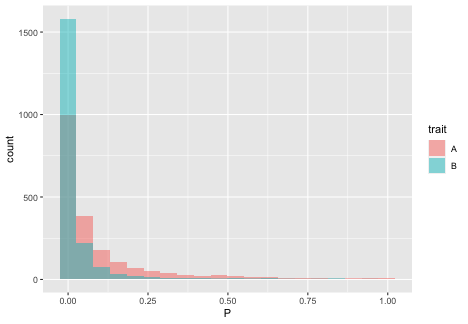
\includegraphics{GWAS-Pvalues_files/figure-latex/visualization-1.png}

Based on the figure above, we can conclude that the distribution of p
values in trait B is stochastically smaller than the distribution in
trait A, even if their underlying \(\beta_G\) are both \(0.3\).
Therefore, it shows that the magnitudes of p-values of different studies
are not directly comparable, unless the generalized linear regression
model being used is the ordinary linear regression model with \(g\)
being identity function.

\clearpage

\hypertarget{bibliography}{%
\section{Bibliography}\label{bibliography}}

\setlength{\parindent}{-0.2in}
\setlength{\leftskip}{0.2in}
\setlength{\parskip}{8pt}

\noindent

\hypertarget{refs}{}
\begin{CSLReferences}{1}{0}
\leavevmode\hypertarget{ref-meta1}{}%
Begum, Ferdouse, Debashis Ghosh, George C. Tseng, and Eleanor Feingold.
2012. {``{Comprehensive literature review and statistical considerations
for GWAS meta-analysis}.''} \emph{Nucleic Acids Research} 40 (9):
3777--84.

\leavevmode\hypertarget{ref-meta2}{}%
Evangelou, Evangelos, and John Ioannidis. 2013. {``Evangelou e,
Ioannidis JP.meta-Analysis Methods for Genome-Wide Association Studies
and Beyond. Nat Rev Genet 14:379-389.''} \emph{Nature Reviews. Genetics}
14 (May).

\leavevmode\hypertarget{ref-MTAG}{}%
Turley, Patrick, Raymond K Walters, Omeed Maghzian, Aysu Okbay, James J
Lee, Mark Alan Fontana, Tuan Anh Nguyen-Viet, et al. 2018.
{``Multi-Trait Analysis of Genome-Wide Association Summary Statistics
Using MTAG.''} \emph{Nature Genetics} 50 (2): 229--37.

\end{CSLReferences}

\end{document}
